% Created 2021-09-12 Sun 22:49
% Intended LaTeX compiler: xelatex
\documentclass[letterpaper]{article}
\usepackage{graphicx}
\usepackage{grffile}
\usepackage{longtable}
\usepackage{wrapfig}
\usepackage{rotating}
\usepackage[normalem]{ulem}
\usepackage{amsmath}
\usepackage{textcomp}
\usepackage{amssymb}
\usepackage{capt-of}
\usepackage{hyperref}
\usepackage[margin=1in]{geometry}
\usepackage{fontspec}
\usepackage{indentfirst}
\setmainfont[ItalicFont = LiberationSans-Italic, BoldFont = LiberationSans-Bold, BoldItalicFont = LiberationSans-BoldItalic]{LiberationSans}
\newfontfamily\NHLight[ItalicFont = LiberationSansNarrow-Italic, BoldFont       = LiberationSansNarrow-Bold, BoldItalicFont = LiberationSansNarrow-BoldItalic]{LiberationSansNarrow}
\newcommand\textrmlf[1]{{\NHLight#1}}
\newcommand\textitlf[1]{{\NHLight\itshape#1}}
\let\textbflf\textrm
\newcommand\textulf[1]{{\NHLight\bfseries#1}}
\newcommand\textuitlf[1]{{\NHLight\bfseries\itshape#1}}
\usepackage{fancyhdr}
\pagestyle{fancy}
\usepackage{titlesec}
\usepackage{titling}
\makeatletter
\lhead{\textbf{\@title}}
\makeatother
\rhead{\textrmlf{Compiled} \today}
\lfoot{\theauthor\ \textbullet \ \textbf{2021-2022}}
\cfoot{}
\rfoot{\textrmlf{Page} \thepage}
\titleformat{\section} {\Large} {\textrmlf{\thesection} {|}} {0.3em} {\textbf}
\titleformat{\subsection} {\large} {\textrmlf{\thesubsection} {|}} {0.2em} {\textbf}
\titleformat{\subsubsection} {\large} {\textrmlf{\thesubsubsection} {|}} {0.1em} {\textbf}
\setlength{\parskip}{0.45em}
\renewcommand\maketitle{}
\author{Houjun Liu}
\date{\today}
\title{Properties of Water}
\hypersetup{
 pdfauthor={Houjun Liu},
 pdftitle={Properties of Water},
 pdfkeywords={},
 pdfsubject={},
 pdfcreator={Emacs 28.0.50 (Org mode 9.4.4)}, 
 pdflang={English}}
\begin{document}

\maketitle


\section{Properties of water}
\label{sec:org501d3bf}
\subsection{Cohesion}
\label{sec:org45b1859}
\begin{itemize}
\item Individual molecules held up well +
\item Strong surface tension
\end{itemize}

\subsection{Adhesion}
\label{sec:orgf0bbb18}
\begin{itemize}
\item Water attracts other molecules, and it stick to water pretty well

\begin{itemize}
\item If we make water molecules touch another molecules, it will stick to
it and start moving
\item Think: a straw --- a thin straw could draw up water without
additional pressure just by water working its way up using adhesion
\end{itemize}

\item This is how we make "xylum" and "Pholem" happen

\begin{itemize}
\item Water's adhesive force --- and adhesive force only --- is how water
travels upwards from a tree
\item Given that some trees are, em, pretty tall, this means that the
capillaries that the water travel in must be very small
\item A Pico-Gauge could be used to measure the pressures within the
phorlem
\end{itemize}
\end{itemize}

\subsection{Water\ldots{}}
\label{sec:orgb0a0992}
\begin{itemize}
\item is wet => Strong tetrahedral H-Bonds
\item is sticky => Has both Cohesive and Adhesive Properties
\item have a \textbf{high specific heat capacity.}

\begin{itemize}
\item Strong bonds
\item Resistant to change
\end{itemize}
\end{itemize}

\subsection{Water's Universal Solvent Properties}
\label{sec:orga2d197e}
Water has high solubility

\begin{itemize}
\item Many things could dissolve in water
\item Makes chemical processes quite easily
\item Quite versatile --- could dissolve stuff easily
\end{itemize}

\subsection{Hydrophillic + Hydrophobic Effects of Water}
\label{sec:org8b5c4b5}
\begin{figure}[htbp]
\centering
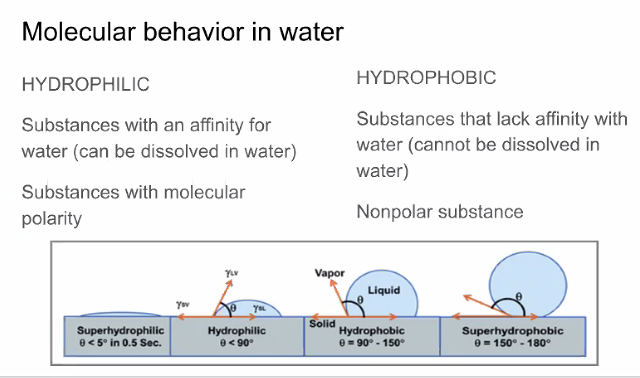
\includegraphics[width=.9\linewidth]{./2020BIO101/Screen Shot 2020-08-26 at 3.07.53 PM.png}
\caption{Screen Shot 2020-08-26 at 3.07.53 PM.png}
\end{figure}

\begin{itemize}
\item In hydrophillic senarios, water will to "puddle out" ("Wetting") ---
adheses to the surface
\item In hydrophobic senarios, water leverage its cohesion properties to
create spheres
\end{itemize}
\end{document}
